% Author:Zhuming Shi, Peking University
% Theme from https://github.com/matze/mtheme

\documentclass[12pt,AutoFakeBold,aspectratio=43,mathserif]{beamer}
\usepackage[english]{babel}

\usetheme{metropolis}

\usepackage{fontspec}% 控制字体
\setmainfont{Times New Roman}% 英文字体
\newfontfamily\arial{Arial}% Arial字体

\usepackage{xeCJK} % 中文支持
\setCJKmainfont{SimSun} % 中文字体
\XeTeXlinebreaklocale "zh"%中文自动换行
\XeTeXlinebreakskip = 0pt plus 1pt%中文自动换行

\usepackage{graphicx}
\usepackage{subfigure}
\usepackage{caption}

\usepackage{amsthm,amsmath,amssymb,mathrsfs}% 数学符号和花体支持
\usepackage{booktabs}% 绘制三线表
\usepackage{latexsym}% 绘制特殊数学符号
\usepackage{siunitx}% 数学模式中使用SI单位

\usepackage[version=3]{mhchem}% 化学反应式
\usepackage{epstopdf}% 插入ChemDraw的.eps结构图

% 代码环境
\usepackage{listings}
\usepackage{color}

\definecolor{dkgreen}{rgb}{0,0.6,0}
\definecolor{gray}{rgb}{0.5,0.5,0.5}
\definecolor{mauve}{rgb}{0.58,0,0.82}

\lstset{frame=tb,
  language=c++,
  aboveskip=3mm,
  belowskip=3mm,
  showstringspaces=false,
  columns=flexible,
  basicstyle={\small\ttfamily},
  numbers=none,
  numberstyle=\tiny\color{gray},
  keywordstyle=\color{blue},
  commentstyle=\color{dkgreen},
  stringstyle=\color{mauve},
  breaklines=true,
  breakatwhitespace=true,
  tabsize=3
}

\setbeamerfont{footnote}{size=\tiny}

\newcommand{\unknow}[1]{{\arial \textbf{#1}}}%未知化合物格式
\newcommand{\substance}[1]{\textbf{\emph{#1}}}%矿物名称格式

% \setbeamertemplate{background}{\includegraphics[height=\paperheight]{figures/misaka1080.png}}

\makeatletter 
\renewcommand{\@thesubfigure}{\hskip\subfiglabelskip}
\makeatother

\title{从控制论到计算机}
\author{前沿第四组}
\date{10月22日}

\begin{document}
    \begin{frame}
        % \frametitle{}
        \titlepage
    
    \end{frame}
    \frame{\frametitle{Outline}\tableofcontents[hideallsubsections]}
    
    \section{机构与变异度}

    \section{调节与控制}

    \section{从控制论到计算机}

    \section*{致谢}

    \begin{frame}
        \frametitle{致谢}
        \begin{columns}
            \begin{column}{.5\linewidth}
                我们的团队(排名不分先后):

                王泽洲\quad 金皓宇\quad 陈齐治
        
                陈思元\quad 李鸿泽\quad 赵晨琪
                
                邓朝萌\quad 谭开云\quad 施朱鸣
            
                \bigskip

                感谢老师们和助教们的帮助!

                祝大家期中顺利,谢谢聆听!
            \end{column}
            \begin{column}{.5\linewidth}
                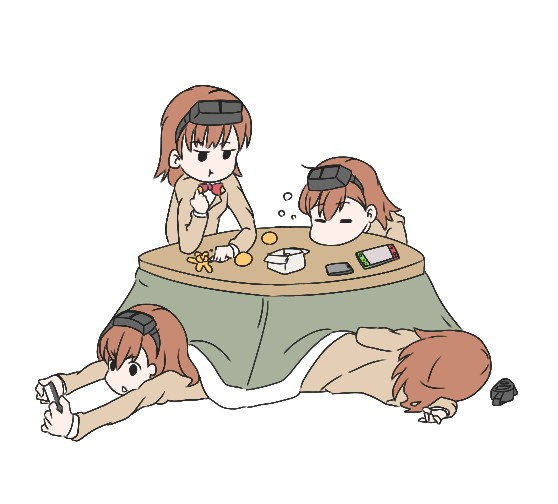
\includegraphics[width=.4\paperwidth]{figures/misaka558.jpg}
            \end{column}
        \end{columns}
        *\footnote{组长邮箱:shizhuming@pku.edu.cn \\ LaTeX代码开源在https://github.com/ShiZhuming/pku-cybernetics}
    \end{frame}
    
\end{document}